\documentclass{article}

\usepackage{graphicx}
\usepackage{tikz}
\usepackage{tikzsymbols}
\usetikzlibrary{calc,patterns,shapes.geometric}
\pagestyle{empty}
\usepackage[margin=0pt]{geometry}
\geometry{papersize={14in,12in}}

\def\centerarc[#1](#2)(#3:#4:#5){\draw[#1] ($(#2)+({#5*cos(#3)},{#5*sin(#3)})$) arc (#3:#4:#5);}

\begin{document}
	\begin{figure}
		\centering
		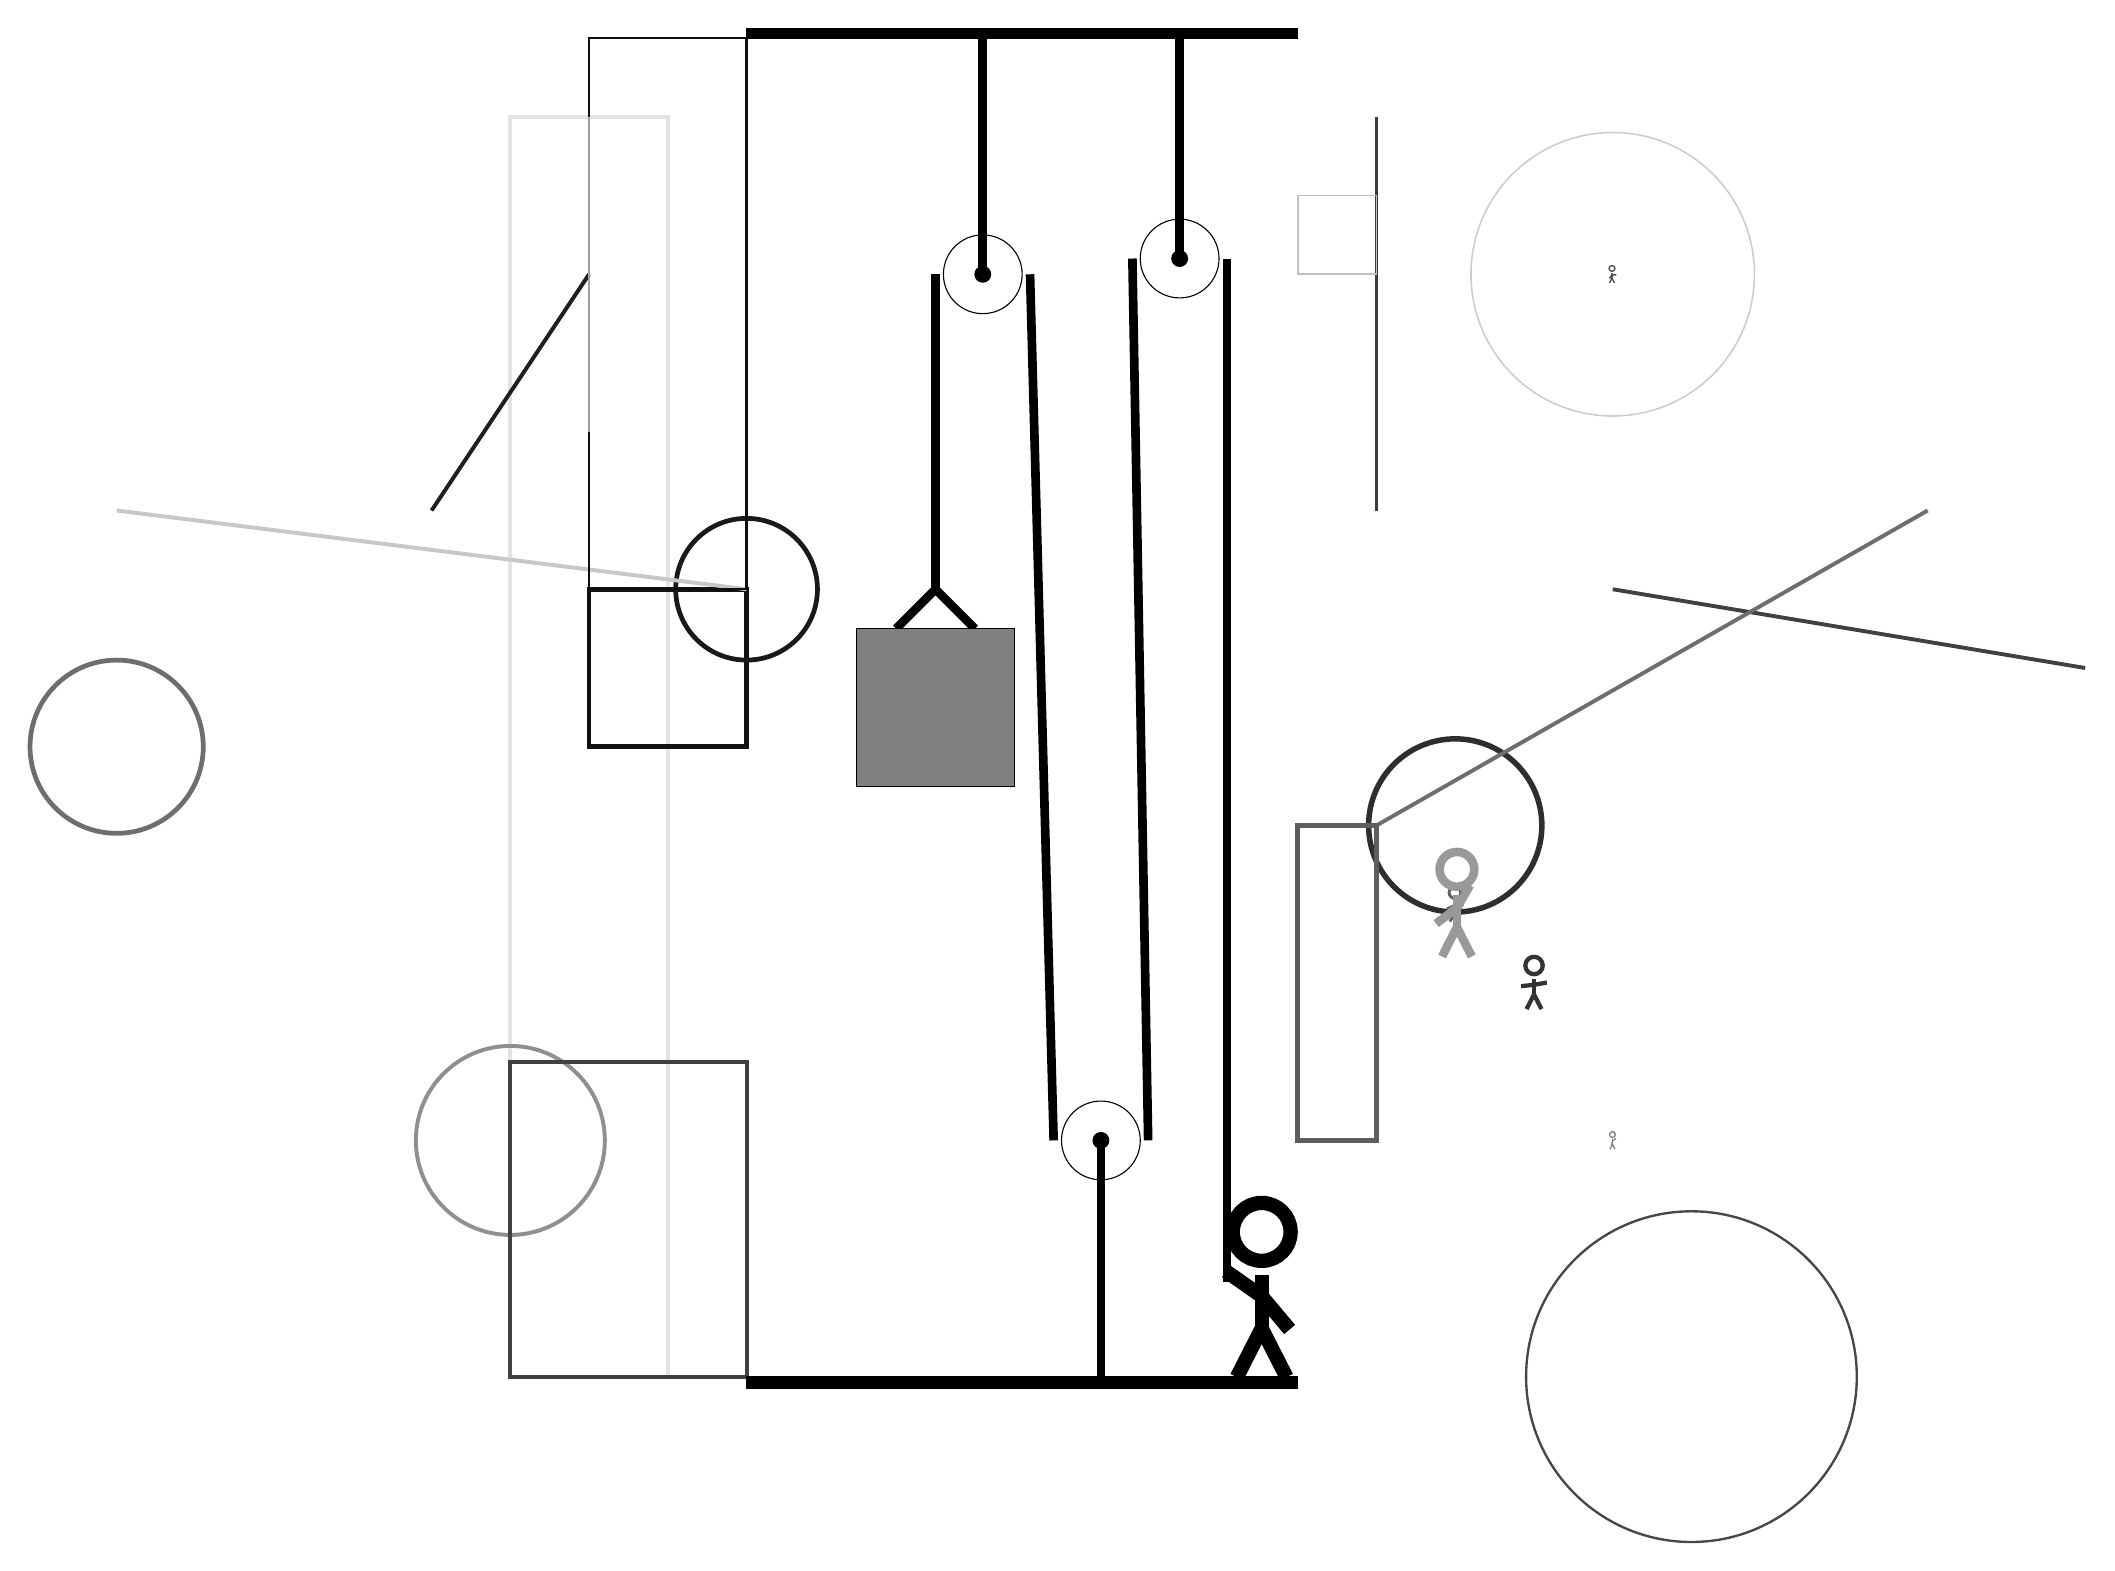
\begin{tikzpicture}
			%%%%% START %%%%%
			
			\draw[fill=black] (-2, 14) rectangle (5, 14.125);
			
			\draw (1, 11) circle (0.5);
			\draw[fill=black] (1, 11) circle (0.1);
			\draw[line width=1.1mm]  (1, 14) -- (1, 11);
			
			\draw[line width=0.5mm, color=black!75](9, 7) -- (15, 6);
			
			\draw[line width=0.5mm, color=black!11] (-3, -3) rectangle (-5, 13);
			\node[line width=0.6mm, color=black!67] at (9, 11) {\Strichmaxerl[1][54][1]};
			\draw[line width=0.5mm, color=black!77](6, 13) -- (6, 8);
			
			\node[line width=0.2mm, color=black!62] at (7, 3) {\Strichmaxerl[2][23][5]};
			\draw[line width=0.6mm, color=black!93] (-2, 5) rectangle (-4, 7);
			
			\draw [line width=0.6mm, color=black!57](-10, 5) circle (1.1);
			\draw [line width=0.6mm, color=black!90](-2, 7) circle (0.9);
			\draw [line width=0.7mm, color=black!82](7, 4) circle (1.1);
			\draw [line width=0.2mm, color=black!20](9, 11) circle (1.8);
			
			\node[line width=0.3mm, color=black!40] at (7, 3) {\Strichmaxerl[6][37][60]};
			\draw [line width=0.5mm, color=black!44](-5, 0) circle (1.2);
			\draw [line width=0.3mm, color=black!78](-8, 0) circle (0.0);
			
			\draw[line width=0.5mm, color=black!22](-2, 7) -- (-10, 8);
			\draw[line width=0.5mm, color=black!57](6, 4) -- (13, 8);
			\draw[line width=0.3mm, color=black!94] (-4, 14) rectangle (-2, 7);
			
			\draw[line width=0.5mm, color=black!88](-4, 11) -- (-6, 8);
			\draw[line width=0.5mm, color=black!75] (-2, -3) rectangle (-5, 1);
			\draw[line width=0.6mm, color=black!63] (6, 0) rectangle (5, 4);
			
			\node[line width=0.4mm, color=black!47] at (9, 0) {\Strichmaxerl[1][80][38]};
			\node[line width=0.3mm, color=black!80] at (8, 2) {\Strichmaxerl[3][6][10]};
			\draw[line width=0.2mm, color=black!25] (6, 12) rectangle (5, 11);
			\draw[line width=0.2mm, color=black!37] (-4, 9) rectangle (-4, 13);
			\draw [line width=0.3mm, color=black!72](10, -3) circle (2.1);
			
			\draw[fill=white](2.5, 0) circle (0.5);
			\draw[fill=black] (2.5, 0) circle (0.1);
			\draw[line width=1.1mm]  (2.5, -3) -- (2.5, 0);
			
			\draw[fill=white](3.5, 11.2) circle (0.5);
			\draw[fill=black] (3.5, 11.2) circle (0.1);
			\draw[line width=1.1mm] (3.5, 14) -- (3.5, 11.2);
			
			\draw[line width=1.1mm] (-0.1, 6.5) -- (0.4, 7.0) -- (0.9, 6.5);
			\draw[fill=black!50] (-0.6, 6.5) rectangle (1.4, 4.5);
			
			\draw[line width=1.1mm] (0.4, 11) -- (0.4, 7.0);
			\centerarc[line width=1.1mm](1, 11)(0:180:0.6);
			\draw[line width=1.1mm](1.6, 11) -- (1.9, 0);
			\centerarc[line width=1.1mm](2.5, 0)(180:360:0.6);
			\draw[line width=1.1mm](3.1, 0) -- (2.9, 11.2);
			\centerarc[line width=1.1mm](3.5, 11.2)(0:180:0.6);
			\draw[line width=1.1mm](4.1, 11.2) -- (4.1, -1.8);
			
			\node at (4.5, -1.9) {\Strichmaxerl[10][-35][-50]};
			
			\draw[fill=black] (-2, -3) rectangle (5, -3.15);
			
			%%%%% END %%%%%
		\end{tikzpicture}
	\end{figure}	
\end{document}